\section{Cr�er un projet}
\subsection{Page principale}
Nous allons d�tailler dans cette partie le sc�nario de cr�ation d'un projet.
L'enseignant cr�e un projet en cliquant sur le lien {\it Cr�er un projet} dans la zone de lien.
Il existe deux mani�res de cr�er un projet:
\begin{itemize}
\item Soit il reprend un projet qui existe dans la base : lien {\it � partir d'un projet existant dans la base}
\item Soit il en cr�e un nouveau : lien {\it un nouveau projet}
\end{itemize}

\begin{flushleft}
\scalebox{0.5}{\includegraphics{../eps/CreerProjetMain.eps}}\\
{\it Page principale}
\end{flushleft}

\subsection{A partir d'un ancien}
L'enseignant doit s�lectionner un projet dans la base.
Il s�lectionne le projet � l'aide d'une arborescence des enseignements.
Il peut lister les projets des enseignements en cliquant sur les noeuds des enseignements.
Un simple clic sur les projets ouvre l'�diteur pour la cr�ation du nouveau projet.
\begin{flushleft}
\scalebox{0.5}{\includegraphics{../eps/CreerProjAncien_Listing.eps}}\\
{\it Liste des projets existants dans la base tri�s par enseignements}
\end{flushleft}
\newpage
\subsection{Nouveau projet}
Il existe deux mani�res de cr�er un nouveau projet:
\begin{itemize}
\item Soit l'enseignant importe un fichier XML depuis son compte.
Dans ce cas un navigateur permet � l'enseignant d'importer le fichier.
\item Soit il �dite directement le projet dans l'�diteur de bord.
\end{itemize}

\begin{flushleft}
\scalebox{0.5}{\includegraphics{../eps/CreerNewProjMain2.eps}}\\
{\it Page de cr�ation d'un projet} 
\end{flushleft}
\newpage
\subsection{Editeur de bord}
L'enseignant utilise pour la saisie du projet l'�diteur embarqu�, dans la zone de visualisation.

Il existe deux mani�res de r�diger le projet.
\begin{flushleft}
\scalebox{0.5}{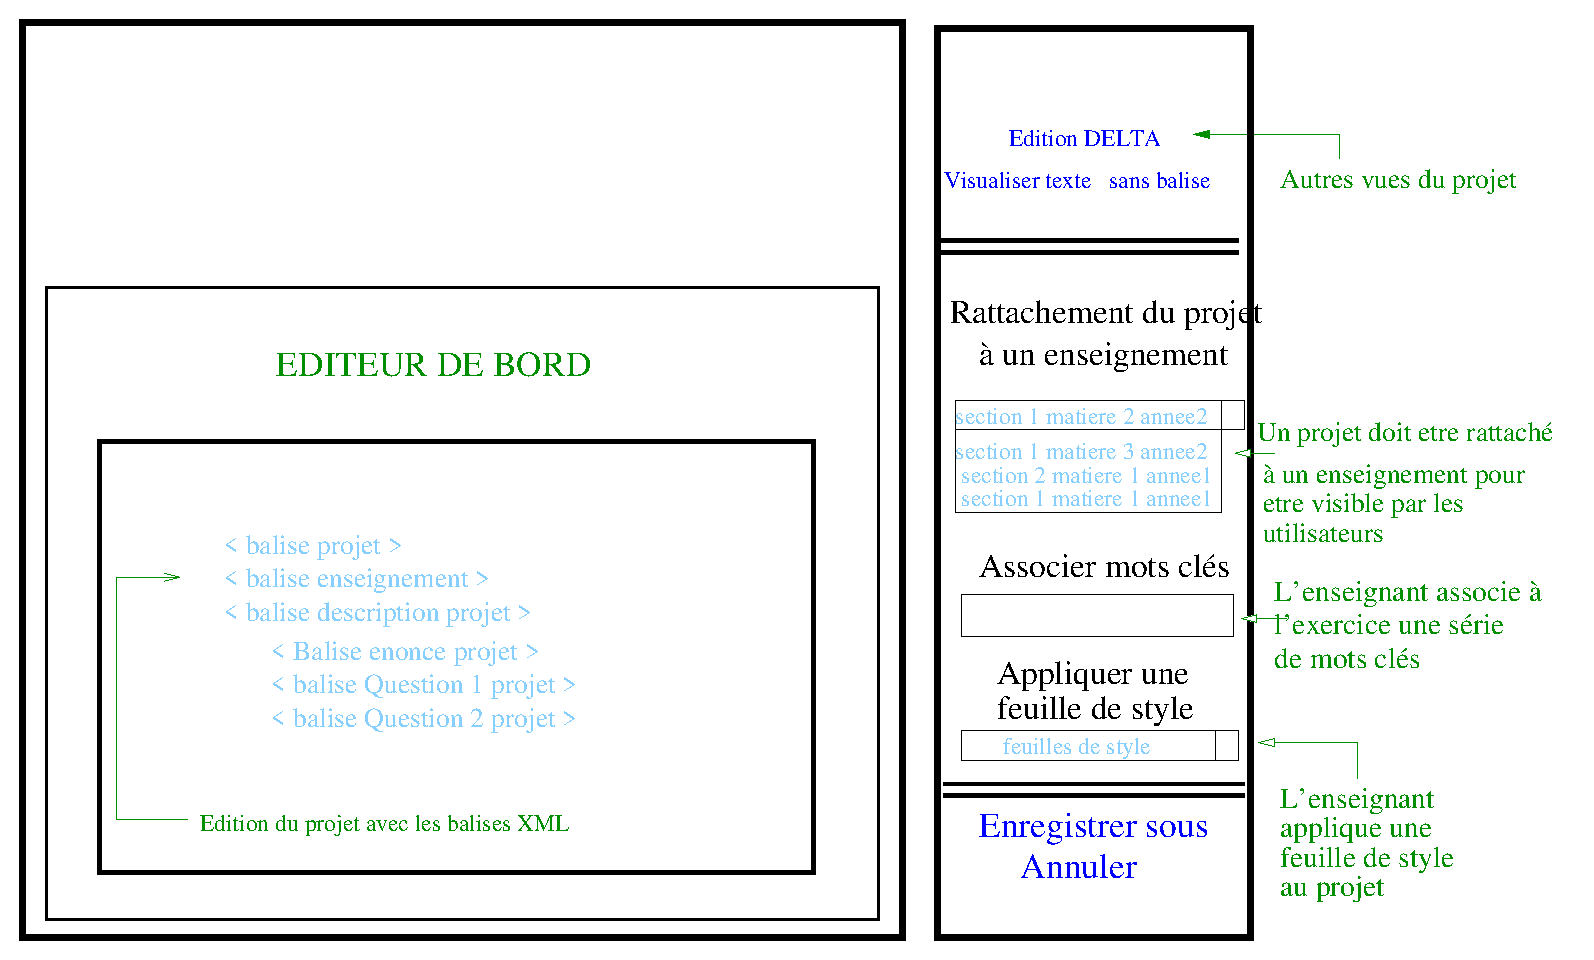
\includegraphics{../eps/projetEditionBalise.eps}}\\
{\it L'enseignant saisie le projet directement en XML}
\end{flushleft}

\begin{flushleft}
\scalebox{0.5}{\includegraphics{../eps/projetEditionSansBalise.eps}}\\
{\it L'enseignant r�dige son projet en mode texte simple (WYSIWYG)}
\end{flushleft}

Une fois le projet saisi, l'enseignant peut rattacher le projet � un enseignement.
Ainsi, le projet sera diffus� dans l'intranet dans les enseignements rattach�s.
Si l'enseignant ne rattache pas le projet � un enseignment, le projet
est stock� dans une zone temporaire.
Les consultants n'auront alors pas acc�s � ce projet.

Une fois le projet r�dig� l'enseignant l'enregistre dans la base :
lien {\it Enregistrer}


